\section{Methodology}
\subsection{The \ang{-45} signal}
\ac{CUPID} aims to generate pure shift spectra by utilising the result of
parametric estimation of \ac{2DJ} data, assumed to take the functional form of
\eqref{eq:jres-fid}.
Instead of estimating successive \ac{1D} \acp{FID}, as proposed by
Nuzillard and Mutzenhardt et al., the entire \ac{2DJ} signal is estimated as a
whole, giving access to the parameter vector $\bth \in \mathbb{R}^{6M}$. With
knowledge of the frequencies and damping factors in both dimensions, it is
possible to generate \iac{FID} which will produce a pure shift spectrum
directly, rather than constructing a full-echo \ac{2DJ} signal, and
subsequently shearing and summing it. The desired signal is named
the ``\ang{-45} signal'' (Figure
\ref{fig:neg-45}), and has the form:
\begin{equation}
    \begin{split}
        \symbf{y}_{\ang{-45}}\left[ \ntwo \right] =
            \sum_{m=0}^{M-1} \bdam \exp \left(\iu \bdphim \right)\\
            \exp\left(
                \left(
                    2 \pi \iu \left(\bdftwom - \bdfonem - \fofftwo\right)
                    - \bdetatwom
                \right) \ntwo \Dttwo
            \right)
    \end{split}
    \label{eq:neg-45}
\end{equation}
$\forall \ntwo \in \lbrace 0, \cdots, \Ntwo - 1 \rbrace$. The \ang{-45} signal
takes the same functional form as a typical \ac{1D}
\ac{FID} acquired by a pulse-acquire experiment, except that the frequency of
each oscillator, which would usually be $\ftwo$, is replaced with $\ftwo -
\fone$. In a \ac{2DJ} experiment, $\fone$ corresponds to the displacement of a
given oscillator from the central frequency of the multiplet it is associated
with. As such, the oscillators belonging to a given multiplet all provide
a contribution with the same frequency to the \ang{-45} signal, namely the
Larmor frequency of the relevant spin. Construction of the \ang{-45} signal is
effectively a proxy for the shearing and summation procedure used to translate
\ac{2DJ} spectra into pure shift spectra.
\begin{figure}
    \centering
    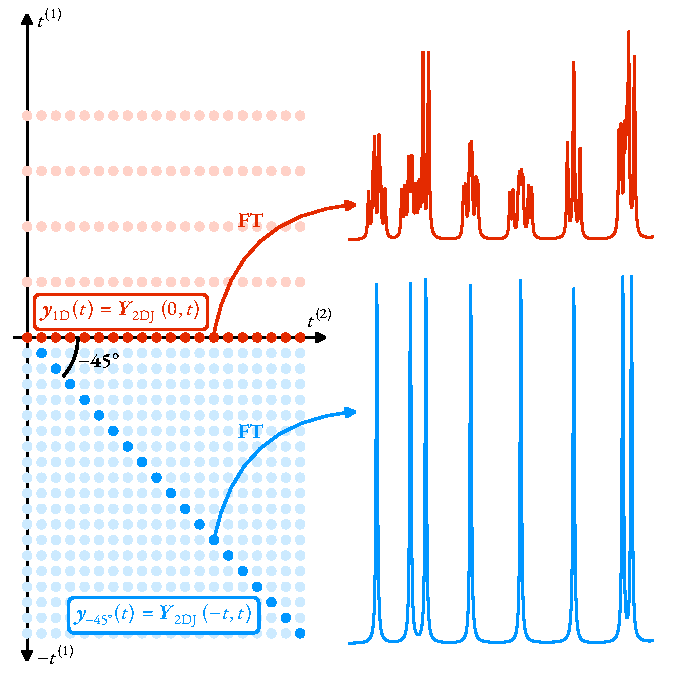
\includegraphics{neg_45_signal/neg_45_signal.pdf}
    \caption[
        An illustration of the reasoning behind the name ``\ang{-45}
        signal'' used to generate pure shift spectra.
    ]{
        An illustration of the reasoning behind the name ``\ang{-45}
        signal'' used to generate pure shift spectra. The pale red dots denote
        a typical \ac{2DJ} \ac{FID}, where
        the amount and rate of sampling in the direct dimension is greater than
        in the indirect dimension (i.e. $\None \ll \Ntwo$ and $\fswone \ll
        \fswtwo$). The bright red dots correspond to the first direct-dimension
        signal $\bY_{\text{2DJ}}(0, \ttwo)$, which has the same form as
        \iac{FID} from a pulse-acquire experiment. A hypothetical signal
        generated by propagating the \ac{FID} into $-\tone$, with the same rate
        of sampling in both dimensions, is denoted with pale blue dots. Taking
        the diagonal of this signal, such that it forms a \ang{-45} angle to the
        $\ttwo$ axis, yields an \ac{FID} $\by_{\ang{-45}}$  which is
        homodecoupled. Note that there is a slight discrepancy
        between \eqref{eq:neg-45} and this description, in that the
        indirect-dimension damping factors $\bdetaone$ are neglected in the
        former case.
    }
    \label{fig:neg-45}
\end{figure}

In using a holistic \ac{2D} estimation routine, as opposed to iteratively
estimating successive \ac{1D} \acs{FID}, a number of benefits are realised.
\begin{itemize}
    \item Multiplet structures which heavily overlap in a conventional \ac{1D}
        dataset become separated in the \ac{2DJ} dataset (assuming that the
        Larmor frequencies of the relevant spins are sufficiently different).
        As such, accurately resolving overlapping multiplets is far more likely
        to be successful with a full \ac{2D} estimation.
    \item With access to the frequencies of each oscillator in both dimensions,
        it is possible to group together those which belong to the same
        multiplet (\emph{vide infra}). Similar information can be obtained by
        extracting slices of a tilted magnitude-mode \ac{2DJ} spectrum at
        appropriate values of $f^{(2)}$, though the lineshapes of peaks suffer
        from the undesirable characteristics described above. The
        \ac{ZS}-\ac{2DJ}\cite{Pell2007} and
        \ac{PSYCHE}-\ac{2DJ}\cite{Foroozandeh2015,Kiraly2017} experiments are
        also able to generate individual multiplet structures, though with
        long \ac{3D} pulse sequences, and with reduced sensitivity relative
        to a conventional \ac{2DJ} experiment.
    \item \note{Others?}
\end{itemize}

The estimation routine used in \ac{CUPID} is as follows:
\begin{enumerate}
    \item Perform appropriate pre-processing on the \ac{2DJ} \ac{FID} in the
        direct dimension: phase correction, and baseline correction if deemed
        to be necessary.
    \item Generate frequency-filtered sub-\acp{FID} for each direct-dimension
        spectral region of interest.
    \item For each sub-\ac{FID}, determine a parameter estimate by applying
        the \ac{MMEMPM} to generate a initial guess, followed by phase
        variance-regularised \ac{NLP}. Optionally, application of the \ac{MDL}
        on the first direct-dimension increment of the \ac{FID} can be used to
        estimate the model order. If the \ac{MDL} is not used, an estimation of
        the model order must be hard-coded.
    \item The pure shift spectrum is generated by combining the parameter
        estimates of each sub-\ac{FID}, generating the \ang{-45} signal with
        \eqref{eq:neg-45}, and performing \ac{FT}.
    \item If of interest, individual multiplet structures can also be generated.
\end{enumerate}

\subsection{Filtration of \ac{2DJ} data}
Unlike the direct-dimension, which can often comprise sparsely distributed
peaks in the Fourier domain, the indirect dimension of \ac{2DJ} datasets tends
to be rather densely populated. As such, it is typically of little use in
attempting to generate filtered sub-\acp{FID} in the indirect dimension. The
filtering procedure utilised for \ac{2DJ} data is therefore an extension of the
filtration procedure for \ac{1D} data described in Section \ref{sec:filtering},
and is depicted in Figure \ref{fig:jres-filtering}. The filtering procedure
involves the following steps:
\begin{enumerate}
    \item The signal $\symbf{Y}_{\text{ve}} \in \mathbb{C}^{\None \times 2 \Ntwo}$ is
    constructed, such that a virtual echo is formed from each direct-dimension
    signal:
    \begin{equation}
        \begin{split}
            \symbf{Y}_{\text{ve}} \left[n^{(1)}\right] =
                &\left[
                \begin{matrix}
                    \Re\left(\symbf{Y}\left[n^{(1)}, 0\right]\right) &
                    \symbf{Y}\left[n^{(1)}, 1\right] &
                    \cdots
                \end{matrix}\right.
                \\
                &\left.
                \begin{matrix}
                    \symbf{Y}\left[n^{(1)}, \Ntwo - 1\right] &
                    0 &
                    \symbf{Y}\left[n^{(1)}, \Ntwo - 1\right]^* &
                    \cdots &
                    \symbf{Y}\left[n^{(1)}, 1\right]^*
                \end{matrix}
                \right]
        \end{split}
    \end{equation}
    $\forall n^{(1)} \in \lbrace 0, \cdots, N^{(1)} - 1 \rbrace$.
    \item $\symbf{Y}_{\text{ve}}$ is subjected to \ac{FT} along the direct
        dimension to produce the spectrum  $\symbf{S}_{\text{ve}}$ (panel a of
        Figure \ref{fig:jres-filtering}). This has an imaginary component of
        zero.
    \item A super-Gaussian $\symbf{G} \in \mathbb{R}^{\None \times 2 \Ntwo}$ is
        constructed (panel b):
        \begin{equation}
            \symbf{G} = \symbf{1} \otimes \symbf{g}^{(2)},
        \end{equation}
        where $\symbf{1} \in \mathbb{R}^{\None}$ is a vector of ones, and
        $\symbf{g}^{(2)}$ is a super-Gaussian vector given by
        \eqref{eq:super-Gaussian-onedim} with $d=2$.
    \item A matrix of additive noise is generated by extracting the variance
        $\sigma^2$ of a strip of $\symbf{S}_{\text{ve}}$ which is devoid of
        peaks, and generating an array $\symbf{W}_{\sigma^2} \in
        \mathbb{R}^{\None \times 2 \Ntwo}$ with values independently sampled
        from a normal distribution with mean $0$ and variance  $\sigma^2$.
    \item The spectrum is filtered according to \eqref{eq:Sve-tilde}, yielding
        $\widetilde{\symbf{S}}_{\text{ve}}$ (panel d).
    \item $\widetilde{\symbf{S}}_{\text{ve}}$ is subjected to \ac{IFT} and is
        sliced in half in the direct dimension, yeilding the final filtered
        signal $\widetilde{\symbf{Y}}$:
        \begin{equation}
            \widetilde{\symbf{Y}} = \IFT^{(2)}\left(\widetilde{\symbf{S}}_{\text{ve}}\right) \left[:, : \Ntwo\right].
        \end{equation}
\end{enumerate}

\begin{figure}
    \centering
    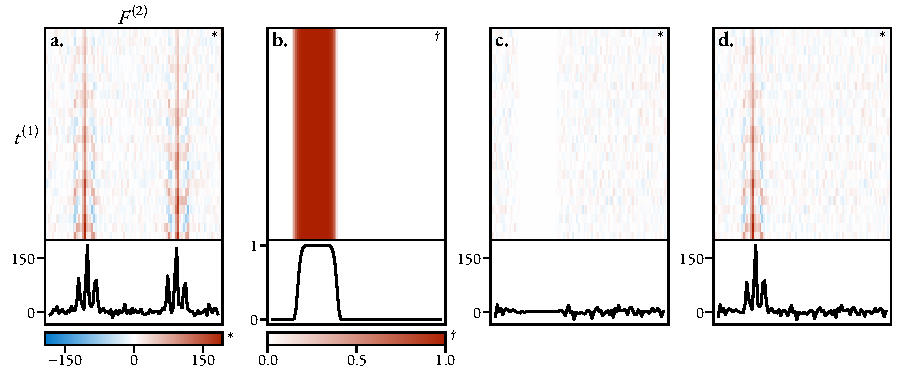
\includegraphics{jres_filtering/jres_filtering.pdf}
    \caption[
        An illustration of the filtering procedure for \ac{2DJ} data.
    ]
    {
        An illustration of the filtering procedure for \ac{2DJ} data.
        For each panel is a heat-map of the full \ac{2D} signal, as well as a
        plot underneath of the first slice of the signal in the direct
        dimension.
        \textbf{a.} The spectrum $\symbf{S}_{\text{ve}}$,
        \textbf{b.} Super-Gaussian filter $\symbf{G}$,
        \textbf{c.} Additive noise, attenuated by the super-Gaussian, $\symbf{W}_{\sigma^2} \odot (\symbf{1} - \symbf{G})$,
        \textbf{d.} Filtered spectrum $\widetilde{\symbf{S}}_{\text{ve}}$
        Panels \textbf{a.}--\textbf{d.} are analogous to panels \textbf{b.}--
        \textbf{e.} in Figure \ref{fig:filtering} for the \ac{1D} case.
    }
    \label{fig:jres-filtering}
\end{figure}


\subsection{Multiplet Prediction}
\ac{CUPID}'s ability to group oscillators present in a parameter set into
multiplet structures relies on knowledge of each oscillator's indirect- and
direct-dimension frequencies. As has already been established, for oscillators
which are associated with the same multiplet, the quantity $\ftwo -
\fone$ should be equal, and is the Larmor frequency of the spin giving rise to
the signals fit by the oscillators. This provides a criterion in order to
assess whether it is likely that two oscillators in the estimation result are
fitting signals which make up the same multiplet:
\begin{equation}
    \left \lvert
        \left( \bdftwo \left[ m_1 \right] -
        \bdfone \left[ m_1 \right] \right) -
        \left( \bdftwo \left[ m_2 \right] -
        \bdfone \left[ m_2 \right] \right)
    \right \rvert < \epsilon
\end{equation}
$\forall m_1, m_2 \in \lbrace 0, \cdots, M-1 \rbrace$, with  $\epsilon \in
\mathbb{R}_{>0}$ being a suitable threshold to account for error in the
estimation and resolution limitations in the dataset. A lower bound on
$\epsilon$ is the spectral resolution in the more poorly resolved dimension,
i.e.  $\epsilon = \min\left(\nicefrac{\fswone}{\None},
\nicefrac{\fswtwo}{\Ntwo}\right)$. However, limitations in resolution due to
signal linewidths and field inhomogeneities can mean that $\epsilon$ has to be
increased beyond this for reasonable multiplet assignments to be achieved.
Algorithm \ref{alg:mp-assign} provides a routine that can be used for multiplet
prediction.

\note{Rethink this bit}
Spurious oscillators:
\begin{itemize}
    \item Very broad, with $\fone \approx \qty{0}{\hertz}$. Caused in cases where very intense signal i.e. from solvent/residual water has a tail which ``breaks into'' the region of interest.
    \item Low intensity, random indirect frequency: overfit: probably fitting a
        noise component
    \item Around region boundary: likely due to artefacts induced by filtering
\end{itemize}
The ability to predict multiplet groupings can also assist in scenarios where
the estimation result contains some oscillators with a spurious nature,
typically due to overfitting. These typically possess either a very large
damping factor or low amplitude, and are not associated with discernible peaks
in the spectrum. Part of the reason that the variance of phases is included in
the fidelity for \ac{NLP} is to try and purge these oscillators, however this
method is not infallible, and undesired oscillators can end up in the final
result. An appreciable number of these can be removed in an automated fashion
by noting that there should not be any oscillators in the estimation result of
a 2DJ dataset which satisfy both of the following:
\begin{enumerate}
    \item The oscillator is not grouped with any other oscillator as part of
        the multiplet assignment.
    \item The magnitude of the indirect dimension frequency of the oscillator
        is appreciably greater than \qty{0}{\hertz}.
\end{enumerate}
These criteria are borne out of the fact that it should not be possible to have
oscillators in a 2DJ dataset which are not part of a multiplet structure,
unless such oscillators are singlets. As no scalar couplings contribute, these
singlets should have an indirect dimension frequency of \qty{0}{\hertz}.
